\section[K. 净化行动 2]{\myboxxi{      \BF{\TT{K}}} 净化行动 2}

\textit{运行时间限制}   2 seconds

\textit{内存使用限制} 1 Gigabyte

\textit{读入文件} \qquad 标准输入

\textit{输出文件} \qquad 标准输出

\begin{quote}
   \textit{如果是王就好了\ldots}
\end{quote}


\subsection{题目描述}

Maddy 仍在清剿 Baddy 的邪恶军团 \ldots

游戏在一个无限大的中国象棋棋盘上进行，棋盘由无数条横线和纵线交叉而成，每个交叉点允许站一个棋子，为了方便表述，我们将其抽象为平面直角坐标系，用二维笛卡尔坐标表示棋子的位置。

Baddy 操控了 $n$ 个黑色的卒棋子和一个黑色的将棋子，这些棋子在游戏过程中固定在它们的初始位置，不会移动。黑卒分别部署在 $(x_1, y_1)$, $(x_2, y_2)$, $\ldots$, $(x_n, y_n)$ 交叉点上，黑将则位于 $(x_\text{K}, y_\text{K})$ 上。

现在 Maddy 操控了一个红色的炮棋子，她可以把红炮部署于棋盘的任意空位置（交叉点），红炮遵循中国象棋的移动规则，具体而言：

\begin{itemize}
   \item 移动，沿着所在横线或纵线移动任意格，但一次移动只能选择横线或纵线，不可同时移动，且不可以跨过同线上其他棋子移动，亦不可以吃子。
   \item 吃子，可以选择同线（横线或纵线）上的敌方棋子作为目标，但中间必须隔着且仅隔着任意一个棋子。吃子后，炮移动到该敌方被吃棋子的位置，被吃的棋子会被移出棋盘。
\end{itemize}

Maddy 在部署红炮后，可以遵循上面的规则连续移动任意次。

Maddy 现在想知道，是否存在一个合理的部署方案和移动红炮的方案，能够最终能吃掉黑将？请帮助她。

\subsection{输入格式}

第一行输入一个整数 $T$ ($1 \le T \le 10^5$), 表示测试数据的数量。

每组测试数据第一行输入 3 个整数 $n$, $x_\text{K}$ 和 $y_\text{K}$ ($0 \le n \le 10^5, -10^9 \le x_\text{K}, y_\text{K} \le 10^9$), 表示黑卒数量和黑将坐标。

随后 $n$ 行，其中第 $i$ 行输入两个整数 $x_i$, $y_i$($-10^9 \le x_i, y_i \le 10^9$), 表示黑卒的位置。

保证所有测试数据输入中的 $\sum n \le 3 \times 10^5$, 保证单组测试数据中所有黑卒的位置两两不同，黑将与任意黑卒的位置均不同。

\subsection{输出格式}

对于每组测试数据，如果存在一个合理的部署方案和移动红炮的方案能够吃掉黑将，则输出一行一个字符串 \texttt{YES}, 否则输出一行一个字符串 \texttt{NO}.

注意评测时不会区分 \TT{YES} 和 \TT{NO} 的大小写，换言之当答案是肯定的时候输出 \TT{yes}, \TT{YES}, \TT{Yes}, \TT{YeS} 等都会被认为是正确的。

\subsection{样例 1}
\begin{minipage}{\linewidth}
   \begin{minipage}[t]{0.49\linewidth}
      \begin{lstlisting}[title=\texttt{standard input}]
3
0 0 0
1 1 1
0 1
4 1 0
0 1
2 1
1 1
1 2
\end{lstlisting}
   \end{minipage}
   \begin{minipage}[t]{0.49\linewidth}
      \begin{lstlisting}[title=\texttt{standard output}]
NO
YES
NO
\end{lstlisting}
   \end{minipage}
\end{minipage}


\subsection{样例 1 解释}

下面的图展示了第 2 组测试数据的黑方棋子位置情况和 Maddy 一种可选的红炮部署位置，也即部署在 $(-2, -1)$, 随后可以直接吃掉黑将。


\begin{figure}[htbp]
   \centering
   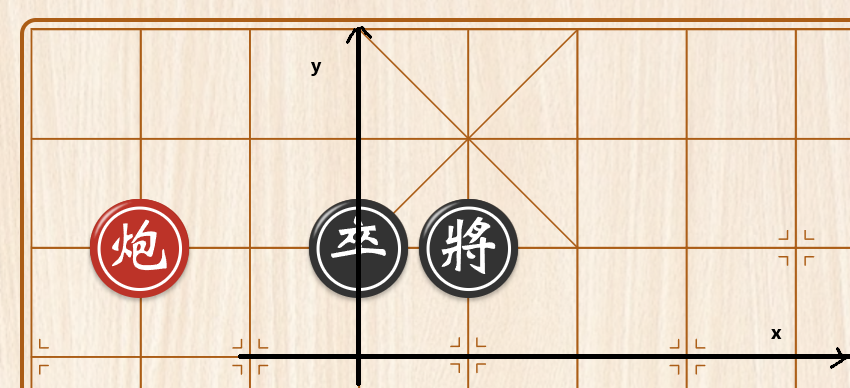
\includegraphics[scale = 0.5]{Problem_K_1.png}
   \caption{第 2 组测试数据的情况}
\end{figure}

下面的图展示了第 3 组测试数据的黑方棋子位置情况。

\begin{figure}[htbp]
   \centering
   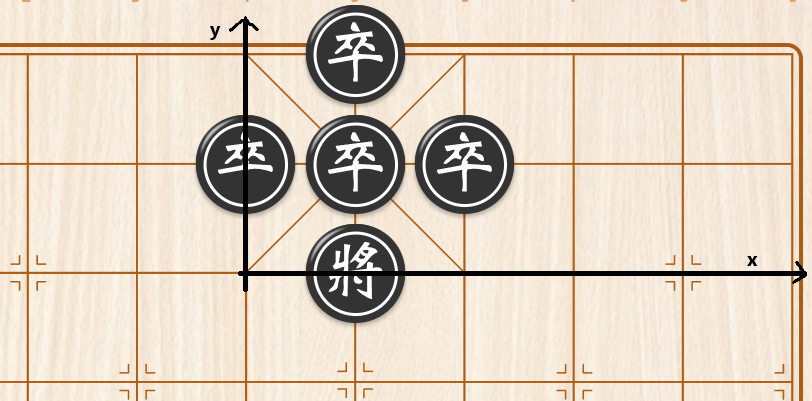
\includegraphics[scale = 0.5]{Problem_K_2.png}
   \caption{第 3 组测试数据的情况}
\end{figure}

请注意，为演示方便，示例图上画出了棋盘边界，但事实上题目描述中已经指出棋盘是无限大的。